本章では,本研究で提案する,歩行と走行の両方を達成することが可能なモデルについて説明する.
これまで提案されてきたモデルでは,歩行運動は倒立振子モデルを用いて説明され,走行運動はバネマスモデルを用いて説明されてきた.
今回提案するモデルは,これら2つのモデルにおける共通項に着目している.
このため,まずそれぞれのモデルについての説明を行う.

\subsection{倒立振子モデル}
まず,歩行モデルである倒立振子モデル(Fig.\ref{ip})について説明する.
倒立振子とは,質量体に,質量を持たず変形しない脚がついたモデルである.
特に,質量体に同じ角度の間隔で脚をつけたモデルをリムレスホイールモデルといい,ヒトの歩行の重心軌道を表すことができる\cite{doi:10.1080/02681119708806242}.
Fig.\ref{rw}にリムレスホイールモデルを表した図を示す.
このモデルの運動は,次式のラグランジュ運動方程式によって説明することができる.
\begin{gather}
  L = \frac{1}{2}J\dot{\theta}^2 - mgl\cos{\theta} \\
 T = \frac{d}{dt}\frac{\partial L}{\partial \dot{\theta}} - \frac{\partial L}{\partial \theta} \\
 J\ddot{\theta} - mgl\sin{\theta} - T = 0 \\
 \frac{d}{dt} \left[
    \begin{array}{cc}
      \theta \\
      \dot{\theta}
    \end{array}
  \right] = \left[
    \begin{array}{cc}
      0 & 1 \\
      \frac{mgl}{J} \sin{\theta} & 0
    \end{array}
  \right] + \left[
    \begin{array}{cc}
      0 \\
     \frac{1}{J}
    \end{array}
  \right]
\end{gather}

ここで,\(L\)はラグラジアン,\(J\)は慣性モーメント,\(g\)は重力加速度である.

このモデルでは,ヒトの歩行において,単脚支持期における重心軌道や,支持脚長がほとんど変化しない点を再現できている.
特に,重心軌道に関しては,単脚支持期には上凸の放物線軌道を,両脚支持期には下凸の放物線軌道の動きを表し,これを周期的に繰り返す.
ここで,両脚支持期は,適切な加速度を与えるための力である,慣性力や蹴り出しの力を与える必要があるため,自発的な運動であるといえる.
逆に,単脚支持期では,与えられた慣性にしたがって重心を移動させる,受動的な運動であると捉えることができる.

\begin{figure}[htbp]
 \centering
 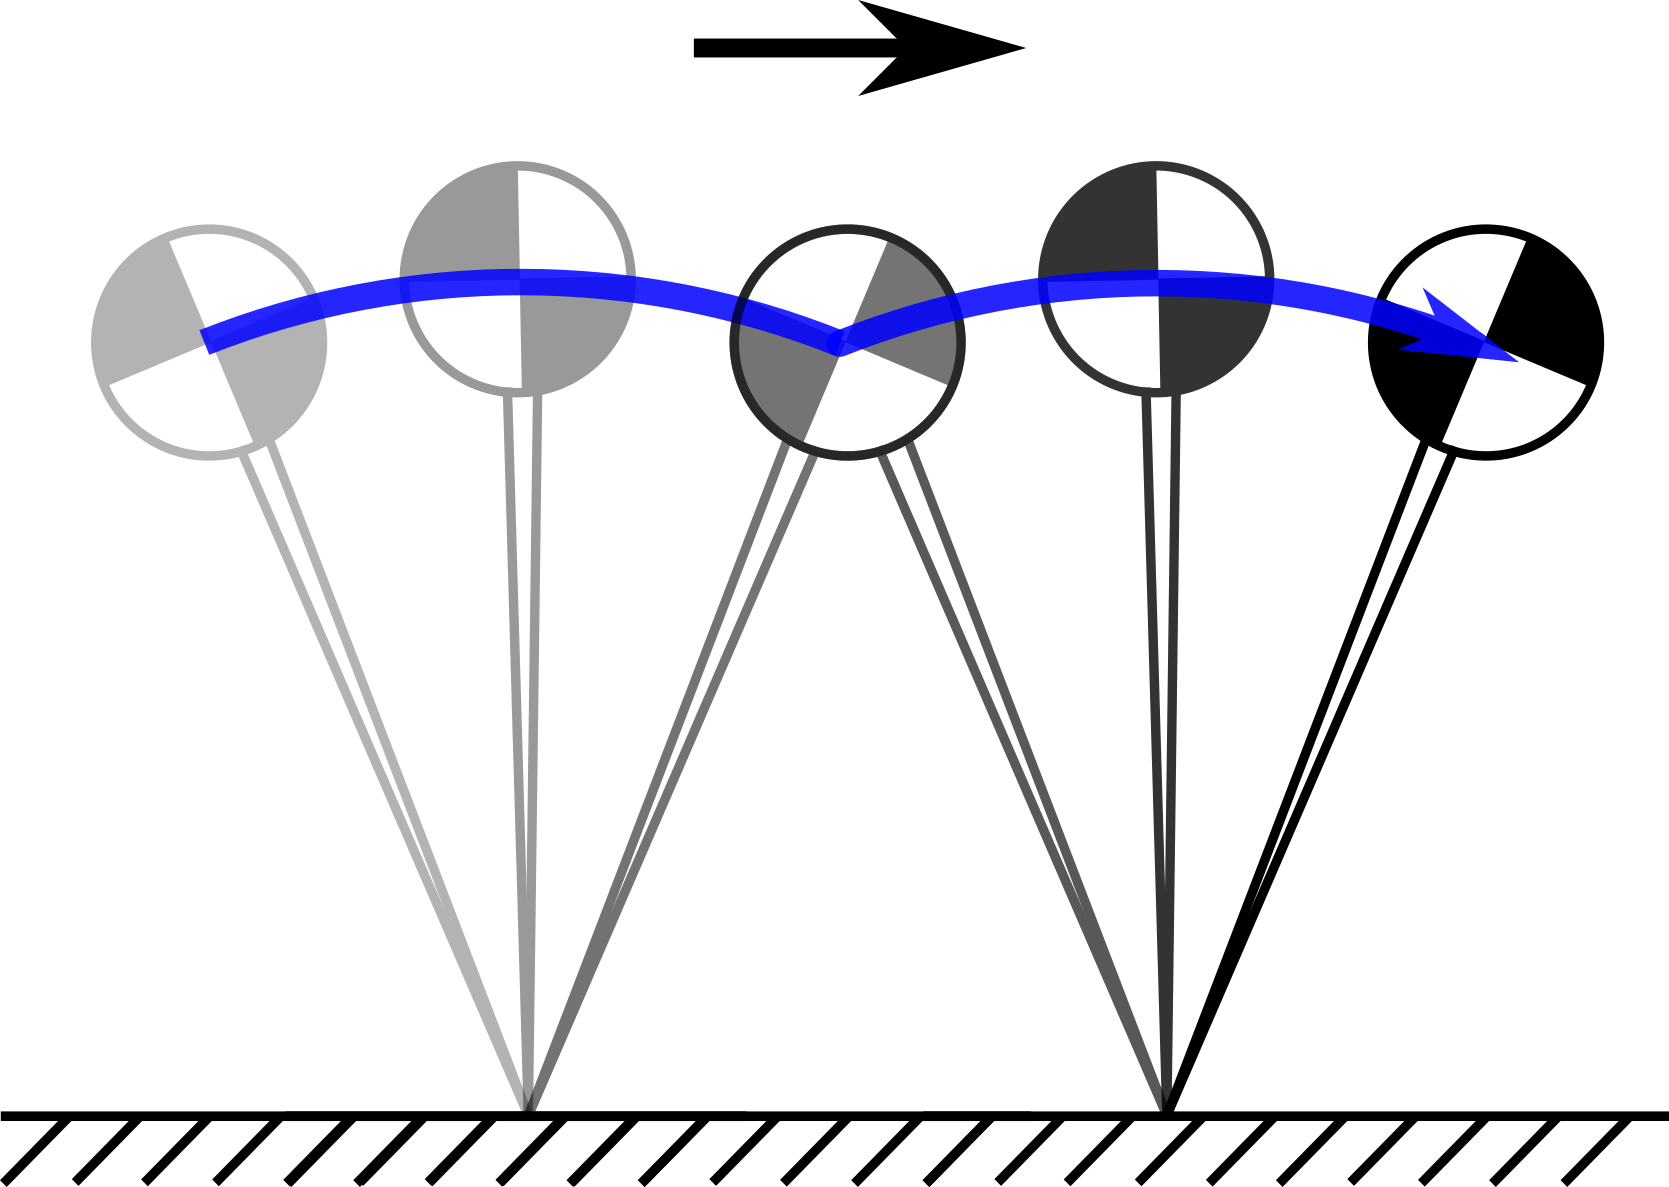
\includegraphics[clip,width=10.0cm]{./fig/inverted_pendulum_walking.png}
    \caption{倒立振子モデル.\label{ip}}
\end{figure}


\begin{figure}[htbp]
 \centering
 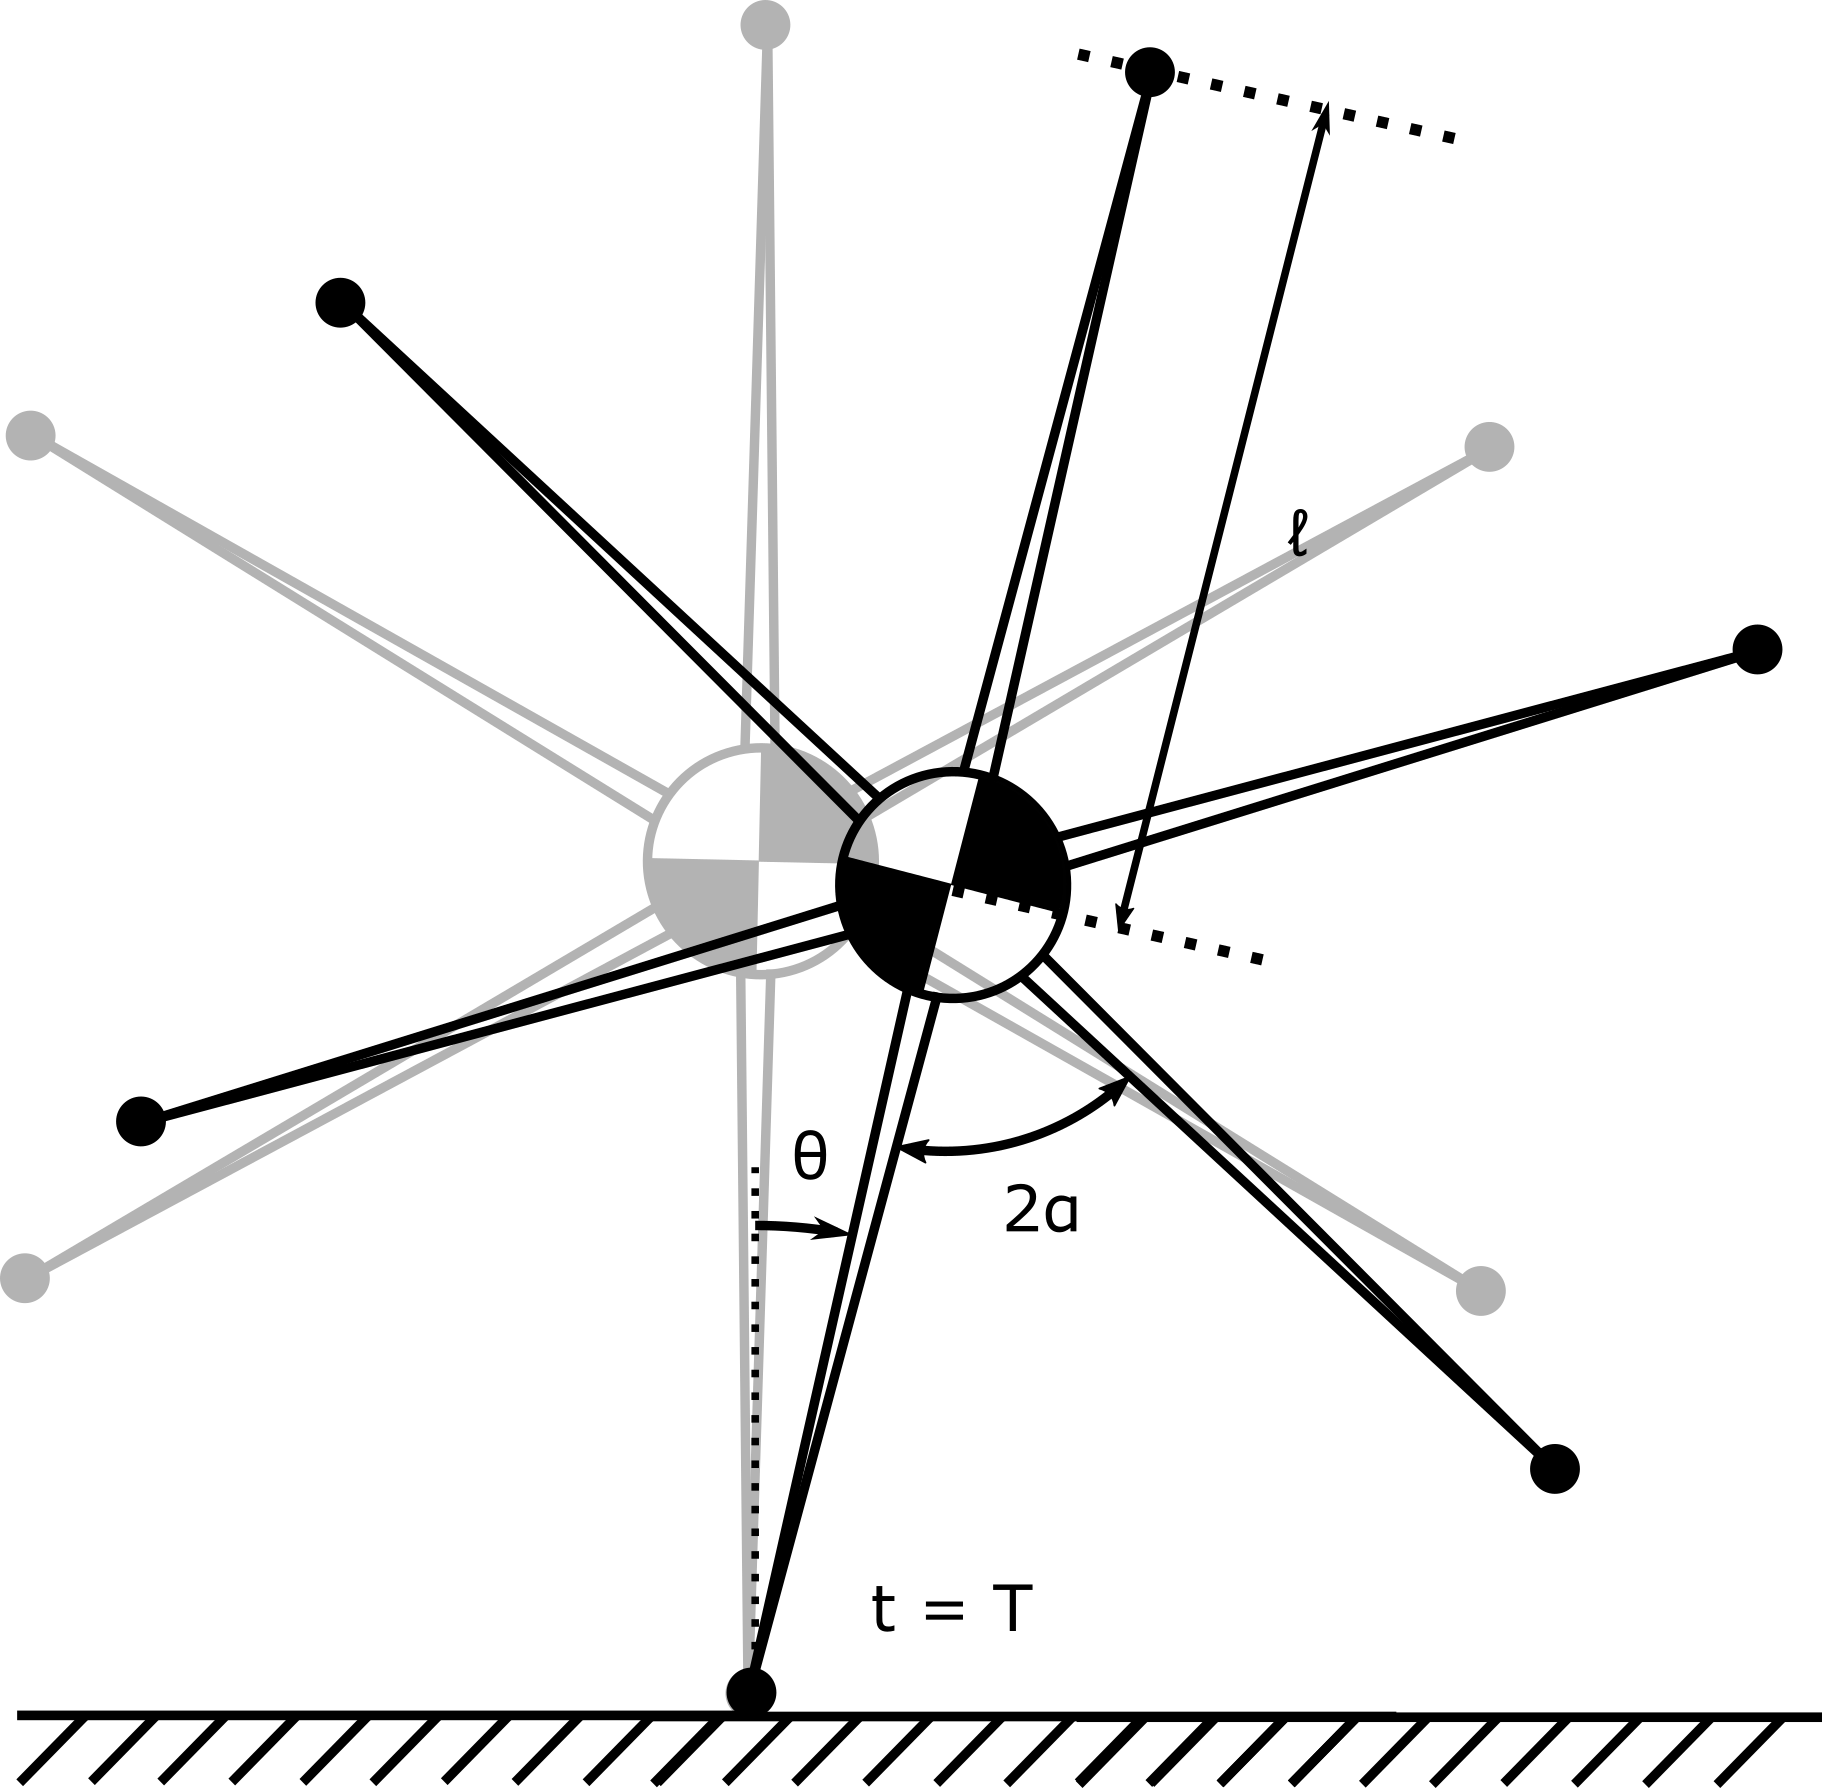
\includegraphics[clip,width=10.0cm]{./fig/rw.png}
    \caption{リムレスホイールモデル.\label{rw}}
\end{figure}



\subsection{バネマスモデル}
次に,走行モデルであるバネマスモデル(Fig.\ref{springmass})について説明する.
このモデルは,質量体に,脚方向に伸縮可能な柔軟なばね脚がついたモデルである.
倒立振子モデルでは,地面に着地したとき脚は変形しない.
それに対し,バネマスモデルでは,着地の際に脚が縮むことで,衝撃を吸収する.
着地の衝撃でばねに蓄えられたエネルギは,離地の際に利用され,跳躍のためのエネルギに変換される.
従来のバネマスモデルの制御手法は,鉛直方向と水平方向の2つに分けて制御を行っている.
鉛直方向の制御は,モデルの跳躍運動に関する制御であり,跳躍運動が脚の伸縮によりもたらされるものであることに着目し,跳躍運動の振幅を安定化させている.
水平方向の制御は,水平方向の移動速度に関する制御であり,接地位置を調節することで,移動速度を一定に保つ.
これらの鉛直方向の制御と水平方向の制御の繰り返しによって,走行を実現することができる.
このときの蹴り出しのために要するばねの力は,鉛直方向の制御則に基づき,次式のエネルギ保存則のように,目標高さによって算出される目標エネルギ\(E_{target}\)と,力学的エネルギによって算出される\(E\)の差によって定義することができる.
\begin{gather}
 E_{target} = mgy_{target} + \frac{1}{2}m \dot{x}_{target}^2 \\
 E = mgy + \frac{1}{2}m \dot{x}^2 + \frac{1}{2}m \dot{y}^2 + \frac{1}{2}kd^2
\end{gather}

ここで,\(y_{target}\)は目標高さ,\(\dot{x}_{target}\)は目標水平速度,\(d\)はばね定数である.
また,バネマスモデルの接地点は,水平速度\(\dot{x}\)と立脚期の長さ\(T_{stance}\)によって,次式で決定される.
\begin{gather}
 x_{f0} = \frac{\dot{x} T_{stance}}{2}
\end{gather}
さらに,この式に誤差訂正のためのPID制御を取り入れた次式によって,一定の速度での歩行が可能となる.
\begin{gather}
 x_{f} = \frac{\dot{x} T_{stance}}{2} + k_{\dot{x}} (\dot{x} - \dot{x_d})
\end{gather}

このときの跳躍時の水平方向の制御は,ばねによる力が働く上凸軌道を描く受動的な運動であり,立脚時の鉛直方向の制御は,慣性によって動く下凸軌道を描く自発的な運動であると考えることができる.

\begin{figure}[htbp]
 \centering
 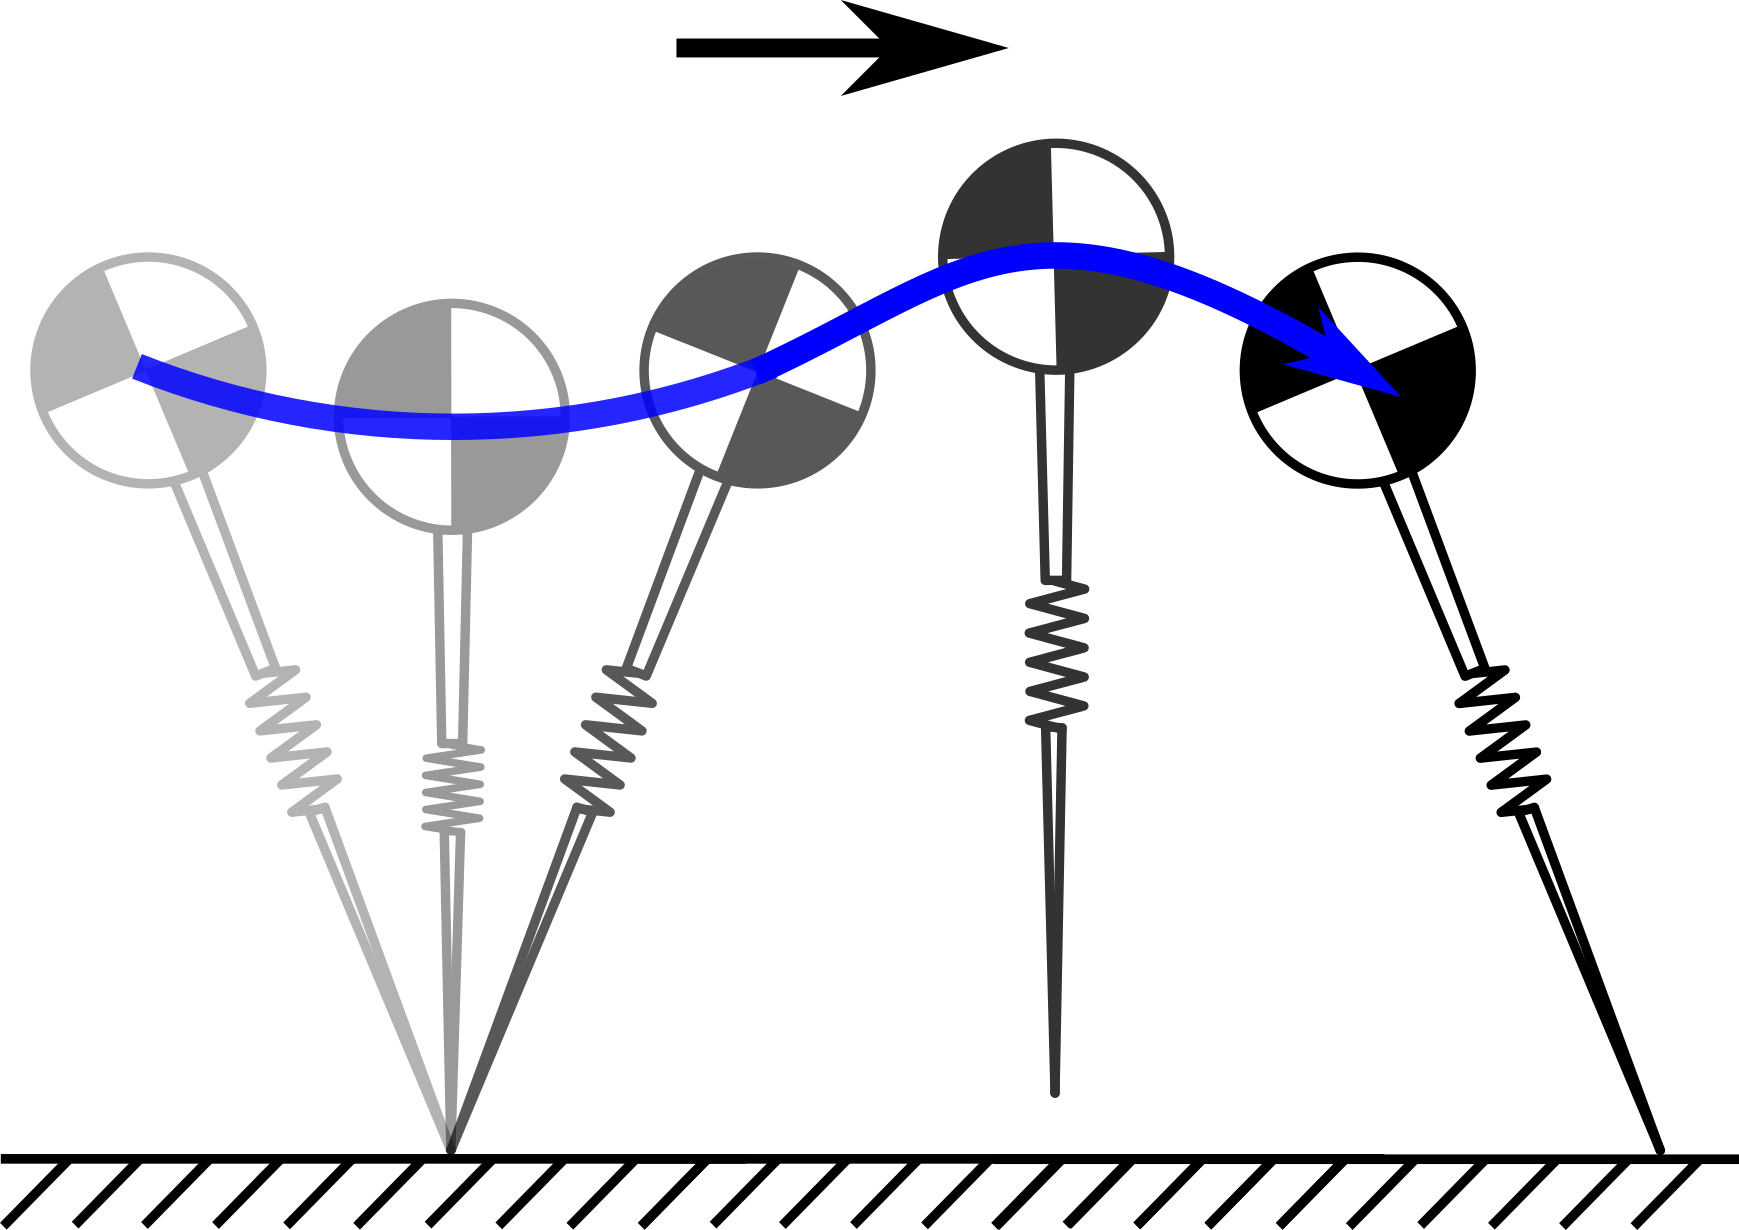
\includegraphics[clip,width=10.0cm]{./fig/slip_running.png}
    \caption{バネマスモデル.\label{springmass}}
\end{figure}



\subsection{提案する脚モデル}
本研究では,歩行時には倒立振子モデルのように振る舞う剛体脚を,走行時にはバネマスモデルのように伸縮可能な脚を同時に表現可能な脚モデルを考案した.
考案した脚モデルの構成をFig.\ref{model}に示す.
この脚構造は,ばね,ばねに作用するためのアクチュエータ,ダンパで構成されている.
また,脚はシリンダ部分とばね脚部分の2つに分かれており,ばね脚部分はシリンダ部分内に含まれている.
シリンダ脚部分は,上部にアクチュエータ,下部にダンパ物質が配置されている.
ばね脚部分には,ばねの上部と下部にストッパがついており,それぞれのストッパは,シリンダ上部にあるアクチュエータやシリンダ下部に接触する,又はどちらとも接触しない状態に変化することでそれぞれ,ばね脚,剛体脚,ダンパ脚のように脚構造の状態を変化させることが可能となっている(Fig.\ref{proposed_model}).
この脚構造の変化によって,歩行時は,シリンダ下部とばね脚の下部ストッパが接触し,後脚の蹴り出しと慣性によって前に進む倒立振子モデルのように振る舞う.
このとき,両脚支持期において,ばね脚部分はシリンダ内部に押し込まれて脚構造が収縮し,単脚支持への移行の際の推進力となる蹴り出し動作を生む.
このため,提案する脚モデルに見られる重心軌道は,倒立振子モデルに見られる両脚支持期の重心軌道とは形状がやや異なった下凸の放物線軌道を描く.
この放物線軌道は,走行動作の支持脚期における下凸の放物線軌道と一致することに注意したい.
また,走行時は,脚の収縮時にばね脚部分がシリンダ内に押し込まれて,シリンダ上部とばね脚の上部ストッパが接触することで,バネマスモデルのように振る舞う.

シリンダ下部にあるダンパ物質は,両脚支持期から単脚支持期への歩行周期の移行の際に重要な役割をもつ.
両脚支持期後期において,後脚は蹴り出しによって重心を押し上げるため,前脚は伸長し,シリンダ下部とばね脚下部ストッパは接触しようとする.
このとき,ダンパ物質が作用することで,接触と同時に発生する跳躍する力を減衰することができ,歩行運動の実現を可能としている.

また,ダンパ物質は,モデルのような直動式の脚構造だけでなく,ヒトのような回転式のリンク構造のにおける歩行の説明においても効果的に機能する.
直動式の脚構造において,脚が伸長するとき,脚方向へは一定の速さで伸長する.
一方,回転式のリンク機構では,関節が屈曲状態から伸展状態に移行するとき,脚方向への伸長率は,脚が伸展するほど低下する.
ダンパ物質を導入することで,直動式の脚構造においても,脚方向への伸長率の低下を再現することができる.

本研究では,このモデルを用いて,歩容を安定させる制御則を導入することで,歩行と走行の歩容の実現を目指す.

\begin{figure}[htbp]
 \begin{minipage}[b]{.5\linewidth}
 \centering
 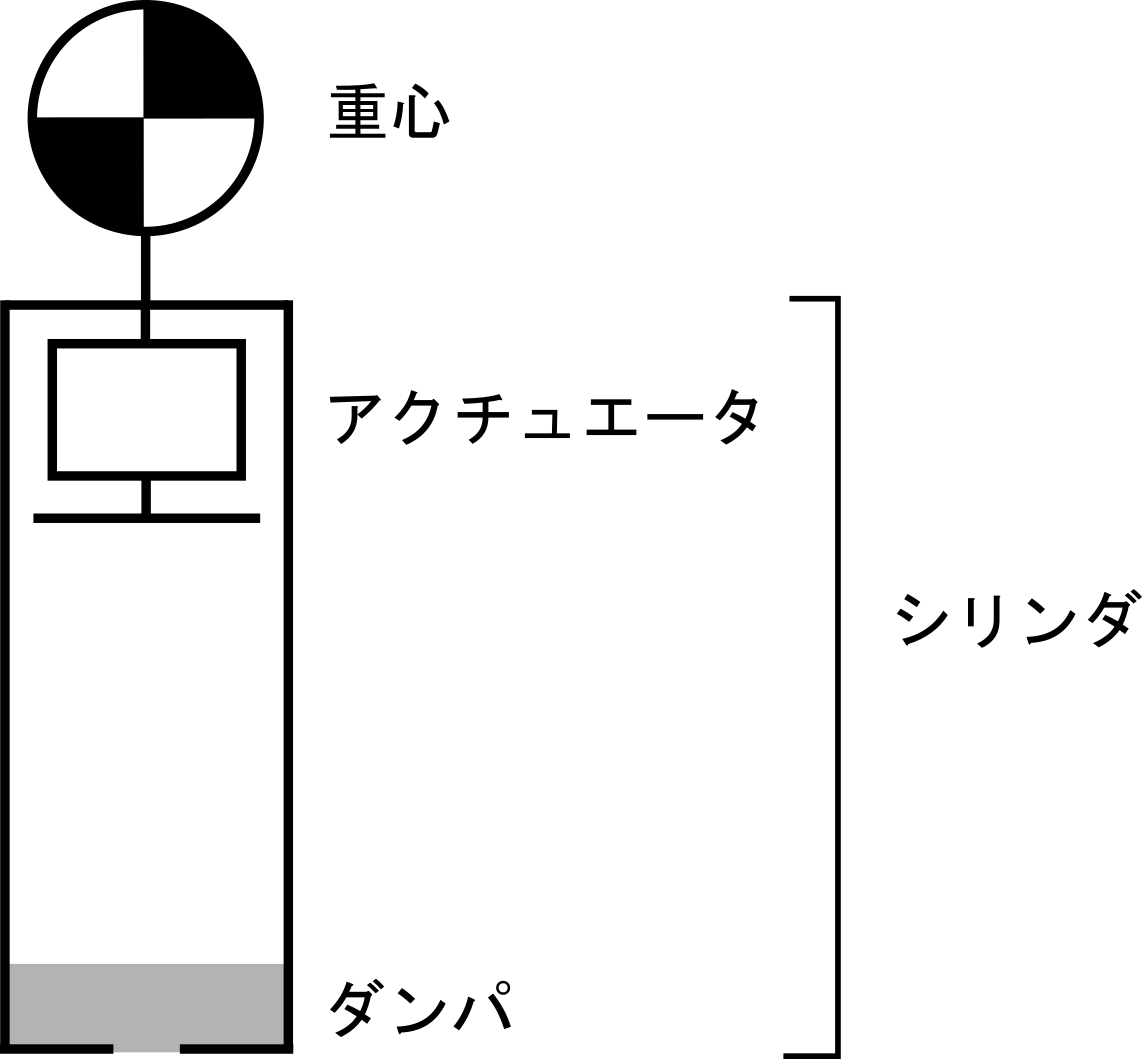
\includegraphics[width = 6.0cm, clip]{./fig/leg_cylinder.png}
 \subcaption{提案する脚モデルのシリンダ部分.\label{leg_cylinder}}
 \end{minipage}
 \begin{minipage}[b]{.5\linewidth}
 \centering
 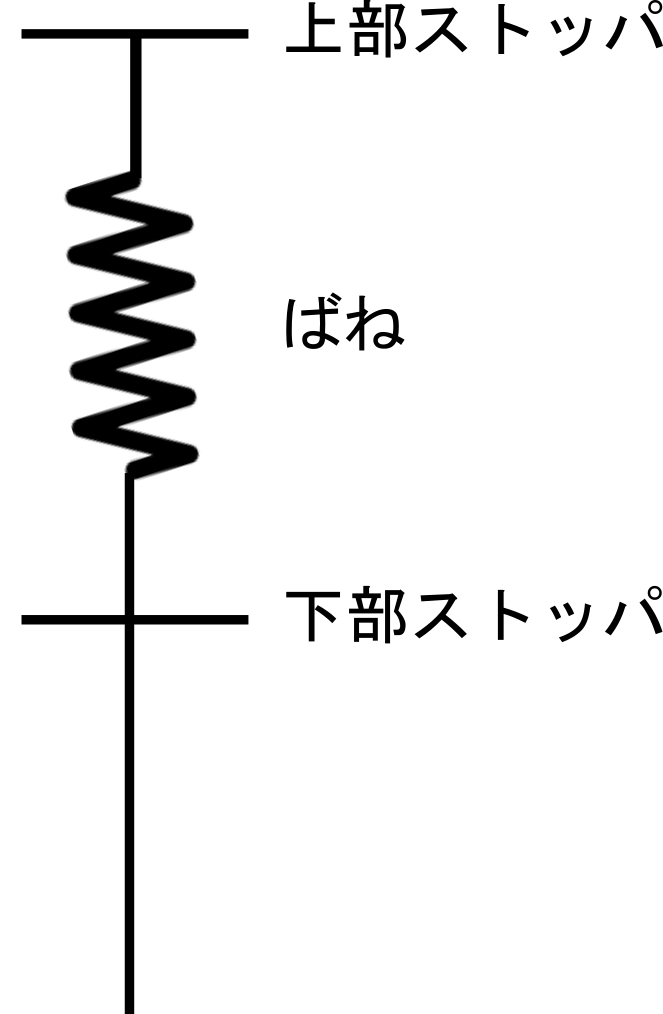
\includegraphics[width = 3.5cm,clip]{./fig/leg_spring.png}
 \subcaption{提案する脚モデルのばね脚部分.\label{leg_spring}}
 \end{minipage}
\caption{提案する脚モデルの構成.実際の運動中には,ばね脚部分はシリンダ部分に内蔵されている.\label{model}}
\end{figure}

\begin{figure}[htbp]
 \centering
 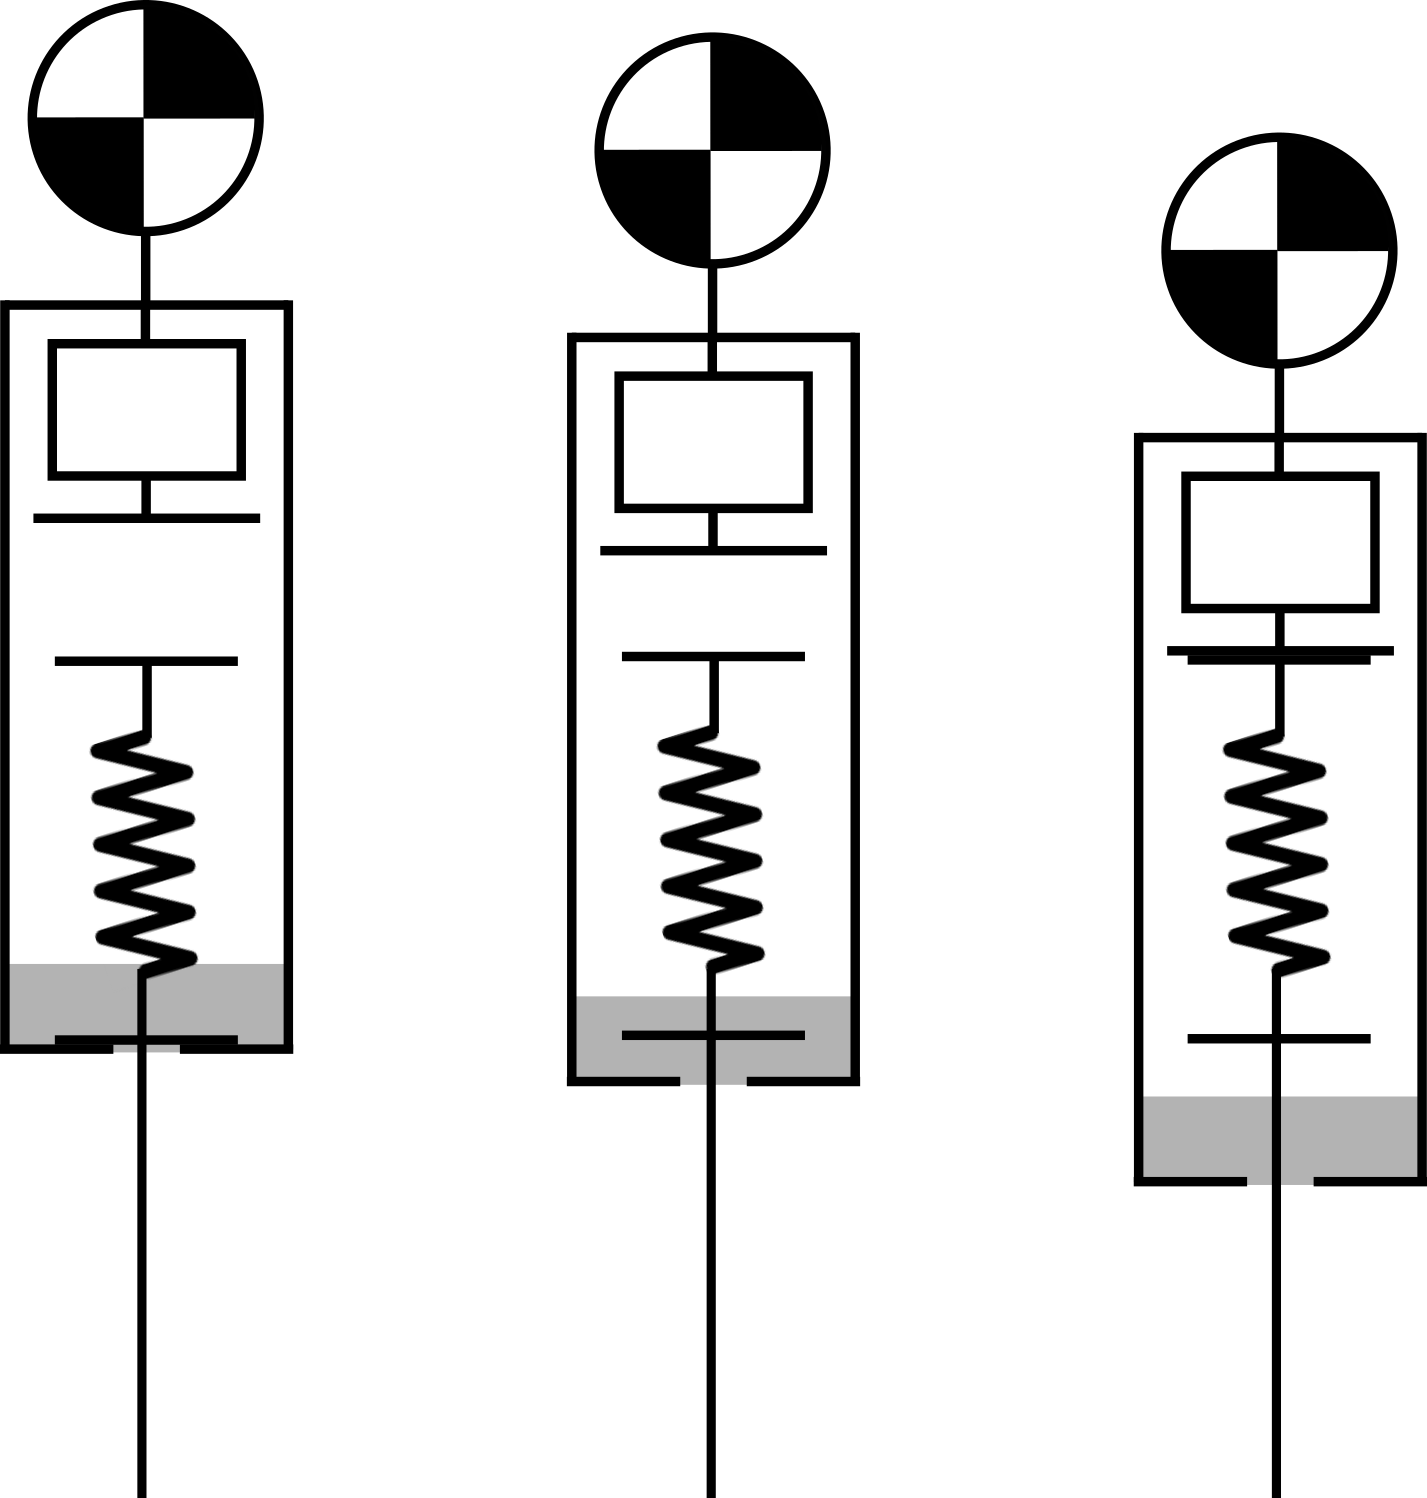
\includegraphics[clip,width=8.0cm]{./fig/leg_concept.png}
    \caption{提案する脚構造の脚状態.左から順番に,剛体脚,ダンパ脚,ばね脚の状態を表している.これらの脚の状態は,ばね脚部分の上部・下部につけられたストッパの位置によって決定される.\label{proposed_model}}
\end{figure}



\subsection{歩容制御アルゴリズム}
提案したモデルの制御則として,前述したバネマスモデルの安定化手法を拡張することを考える.
歩行モデルと走行モデルの2つで単脚支持期における挙動を比較すると,歩行モデルでは,脚の長さが変化しないために上凸軌道を描くのに対し,走行モデルでは,ばねが収縮するために下凸軌道を描く.
この動作の差異が原因で,歩行と走行を同時に表現することは難しい.
しかし,この下凸軌道の自発的運動と上凸軌道の受動的運動の繰り返しの現象は,前述したように,歩行の場合においても同様に見られる現象である(Fig.\ref{compare}).
すなわち,歩行運動と走行運動において,脚の伸縮動作中に水平方向の制御が働くという共通項がある.
この共通項に着目することで,走行における制御則を,歩行に拡張できる可能性があると考えた.

そこで,モデルの制御則として,仮想脚という概念を導入することで,歩行と走行の制御則を一般化することを考えた.
仮想脚の定義として,最大長を任意の長さに設定可能であり,歩行での両脚支持期における中間点にある,収縮可能な脚と仮定する.
仮想脚の脚長を,走行時の実際の脚長と仮定すると,モデルにおける仮想脚と実際の脚の動きは一致し,仮想脚は走行運動の動作を見せる.
歩行時は,仮想脚の自然長が,両脚支持期初期の質量体と各脚の中間点の長さと仮定すると,歩行中の仮想脚は,両脚支持期中は重心が低くなるために,走行動作
支持脚のような振る舞いをする.
また,単脚支持期には,仮想脚は収縮状態から自然長に伸びている状態であり,実際の脚より短い状態であるため,跳躍運動を行う.
これにより,歩行時における仮想脚は,走行動作のように支持脚期と跳躍期を繰り返すように振る舞う.
このように,仮想脚を想定することで,歩行と走行の2つの動作を,仮想脚の走行動作と同様に記述することができる.
走行動作の制御は,バネマスモデルにおいて使用される制御則を用いることで実現できる.
このため,本モデルで,仮想脚を想定し,モデルの仮想的な運動の制御を行う手法を用いる.

ここで,提案するモデルの実際に使用する制御において,実際の走行モデルと異なる,2つの制約条件を考慮する必要がある.
1つ目が,実際の脚と仮想脚の着地タイミングが異なる場合がある点である.
仮想脚を想定したモデルを考えたとき,仮想脚の定義した脚長によって,実際の脚が接地するよりも前に仮想脚が接地する場合が生じ得る.
その場合,実際の脚が接地するまで,仮想脚の位置が接地位置で固定されているものとして制御を行う.
2つ目が,仮想脚の状態の遷移に関する問題である.
単にこのモデルを使用するだけでは,歩行と走行を安定して行うことは可能だが,2つの動作を遷移することはできない.
実際の脚の歩容によって,仮想脚は異なる状態となる可能性を有している.
例えば,歩行動作中の場合,単脚支持期において,仮想脚は跳躍期になる.
一方で,走行動作中の場合,単脚支持期には,仮想脚は単脚支持期である.
このように,動作によって,実際の脚が単脚支持期中であるとき,仮想脚は単脚支持期にも跳躍期にもなりえる.
このため,歩容の遷移を可能とするために,2つの条件を制御に加える.
実際の脚による運動の状態が安定な状態であれば,仮想脚は,跳躍期と単脚支持期を周期的に繰り返す.
しかし,運動の状態が不安定な場合,歩容が歩行から走行に,または走行から歩行に変化する場合がある.
これを考慮するため,仮想脚は,跳躍期と単脚支持期の周期を2回繰り返すことによって,実際の脚の状態に合わせる必要がある.

これらの制約を考慮すると,以下の2つの条件を認める必要がある.

\begin{itemize}
 \item[\labelitemiv] 実際の脚が単脚支持期に移行したとき,仮想脚も別の状態に移行する.
 \item[\labelitemiv] 実際の脚が両脚支持期であるとき,仮想脚は単脚支持期に移行する.
\end{itemize}

これらの制約条件を制御則に組み込むことによって,歩容の遷移が可能になり,モデルでの歩行と走行の安定性を説明できるようになる.


\begin{figure}[htbp]
 \centering
 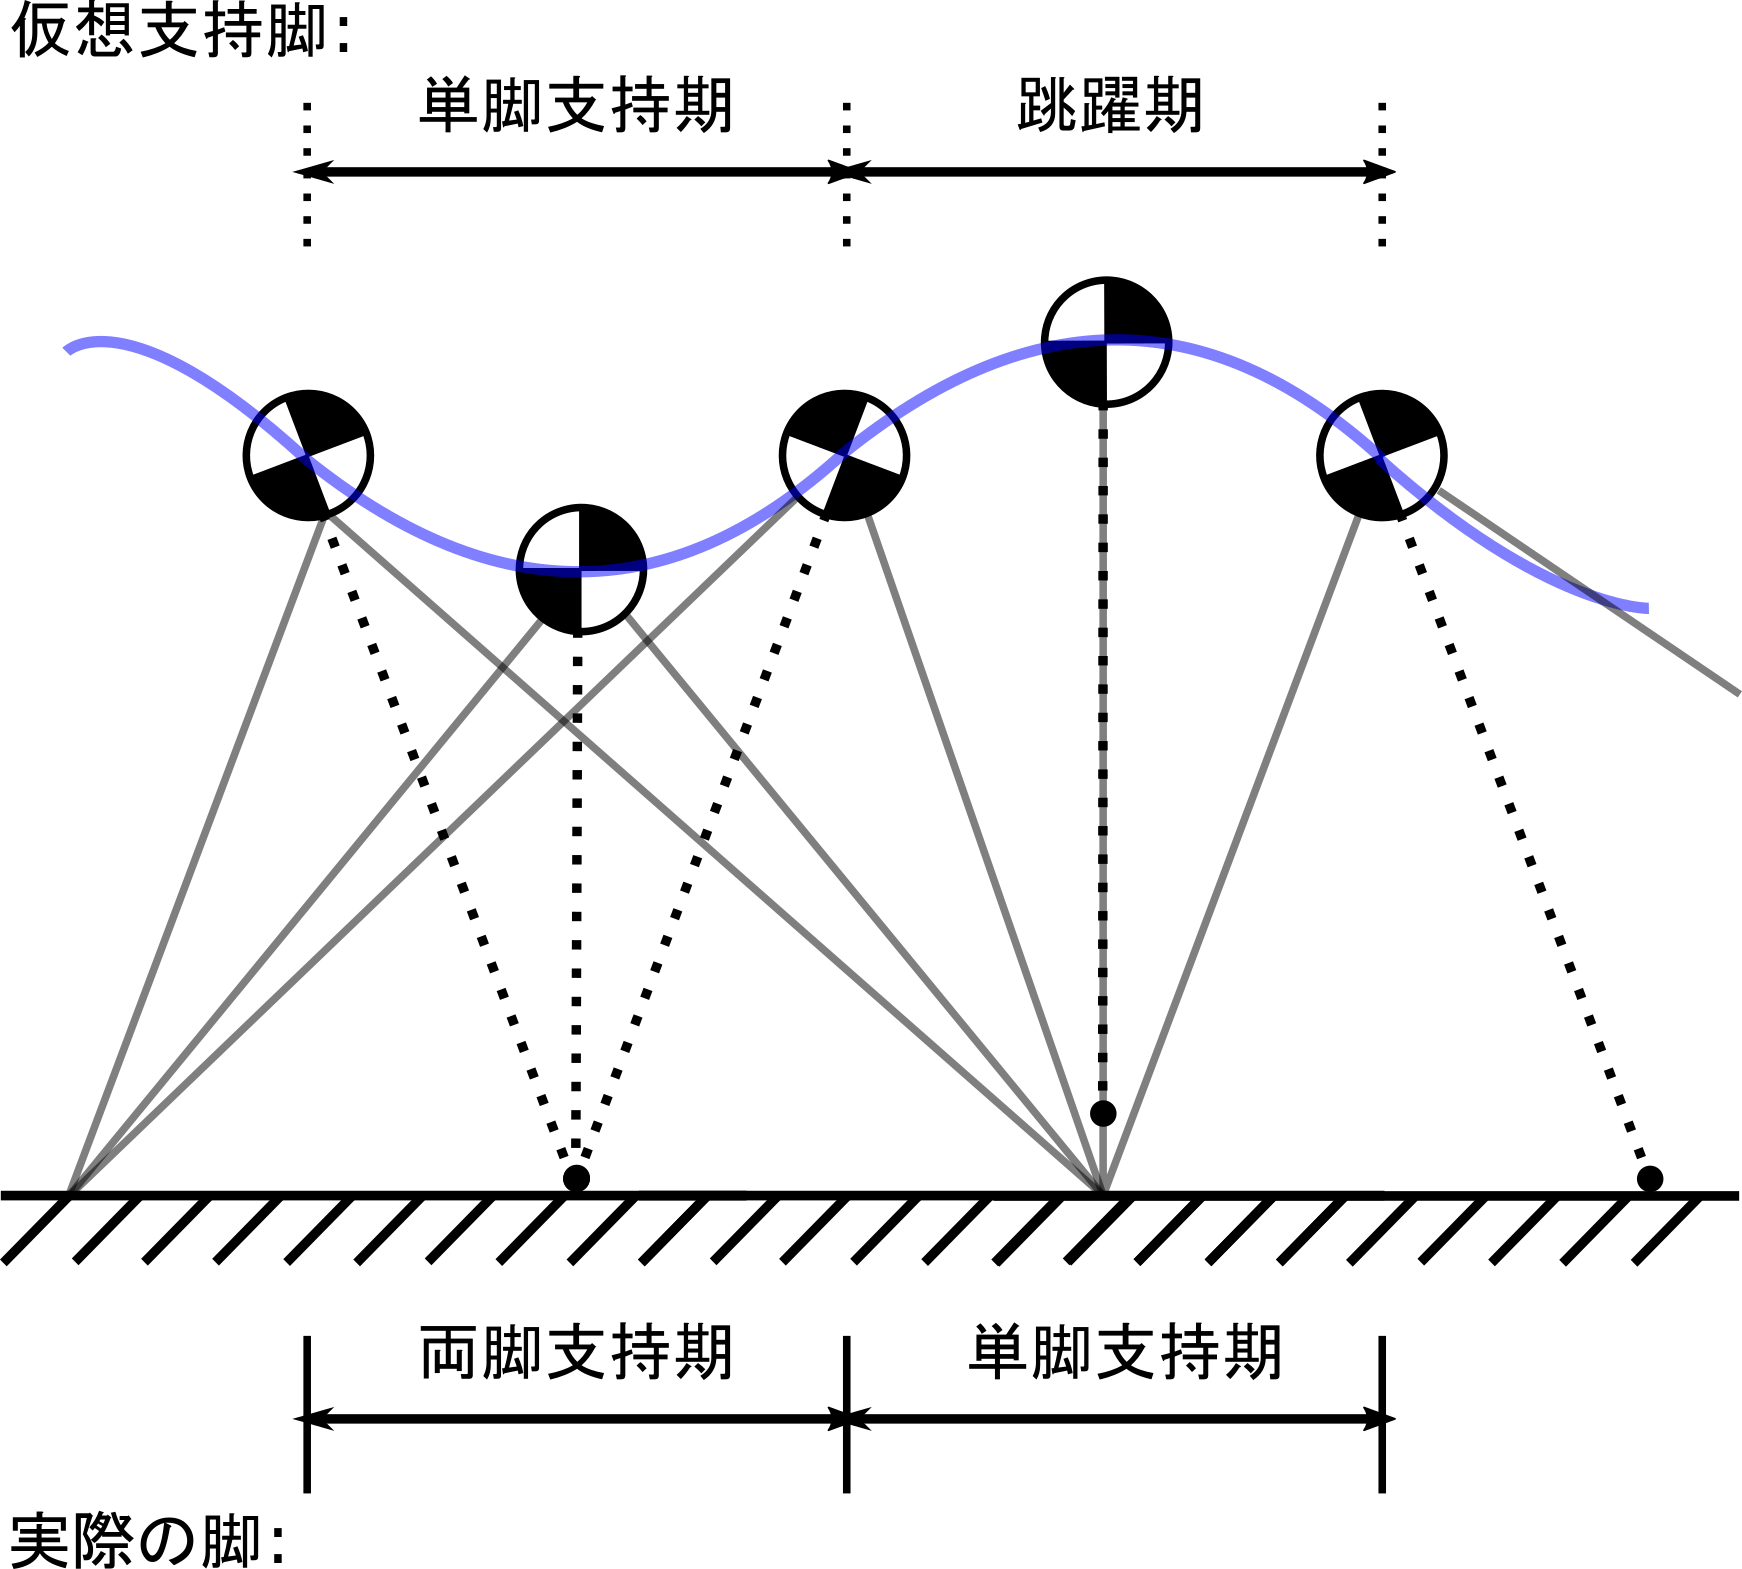
\includegraphics[width = 10.0cm, clip]{./fig/walking_with_vsl.png}
 \caption{歩行動作に仮想脚を導入した場合.青色の曲線は重心軌跡を,黒色の線は脚を,黒色の点線は仮想脚を表している.\label{w_vsl}}
\end{figure}
\begin{figure}
 \centering
 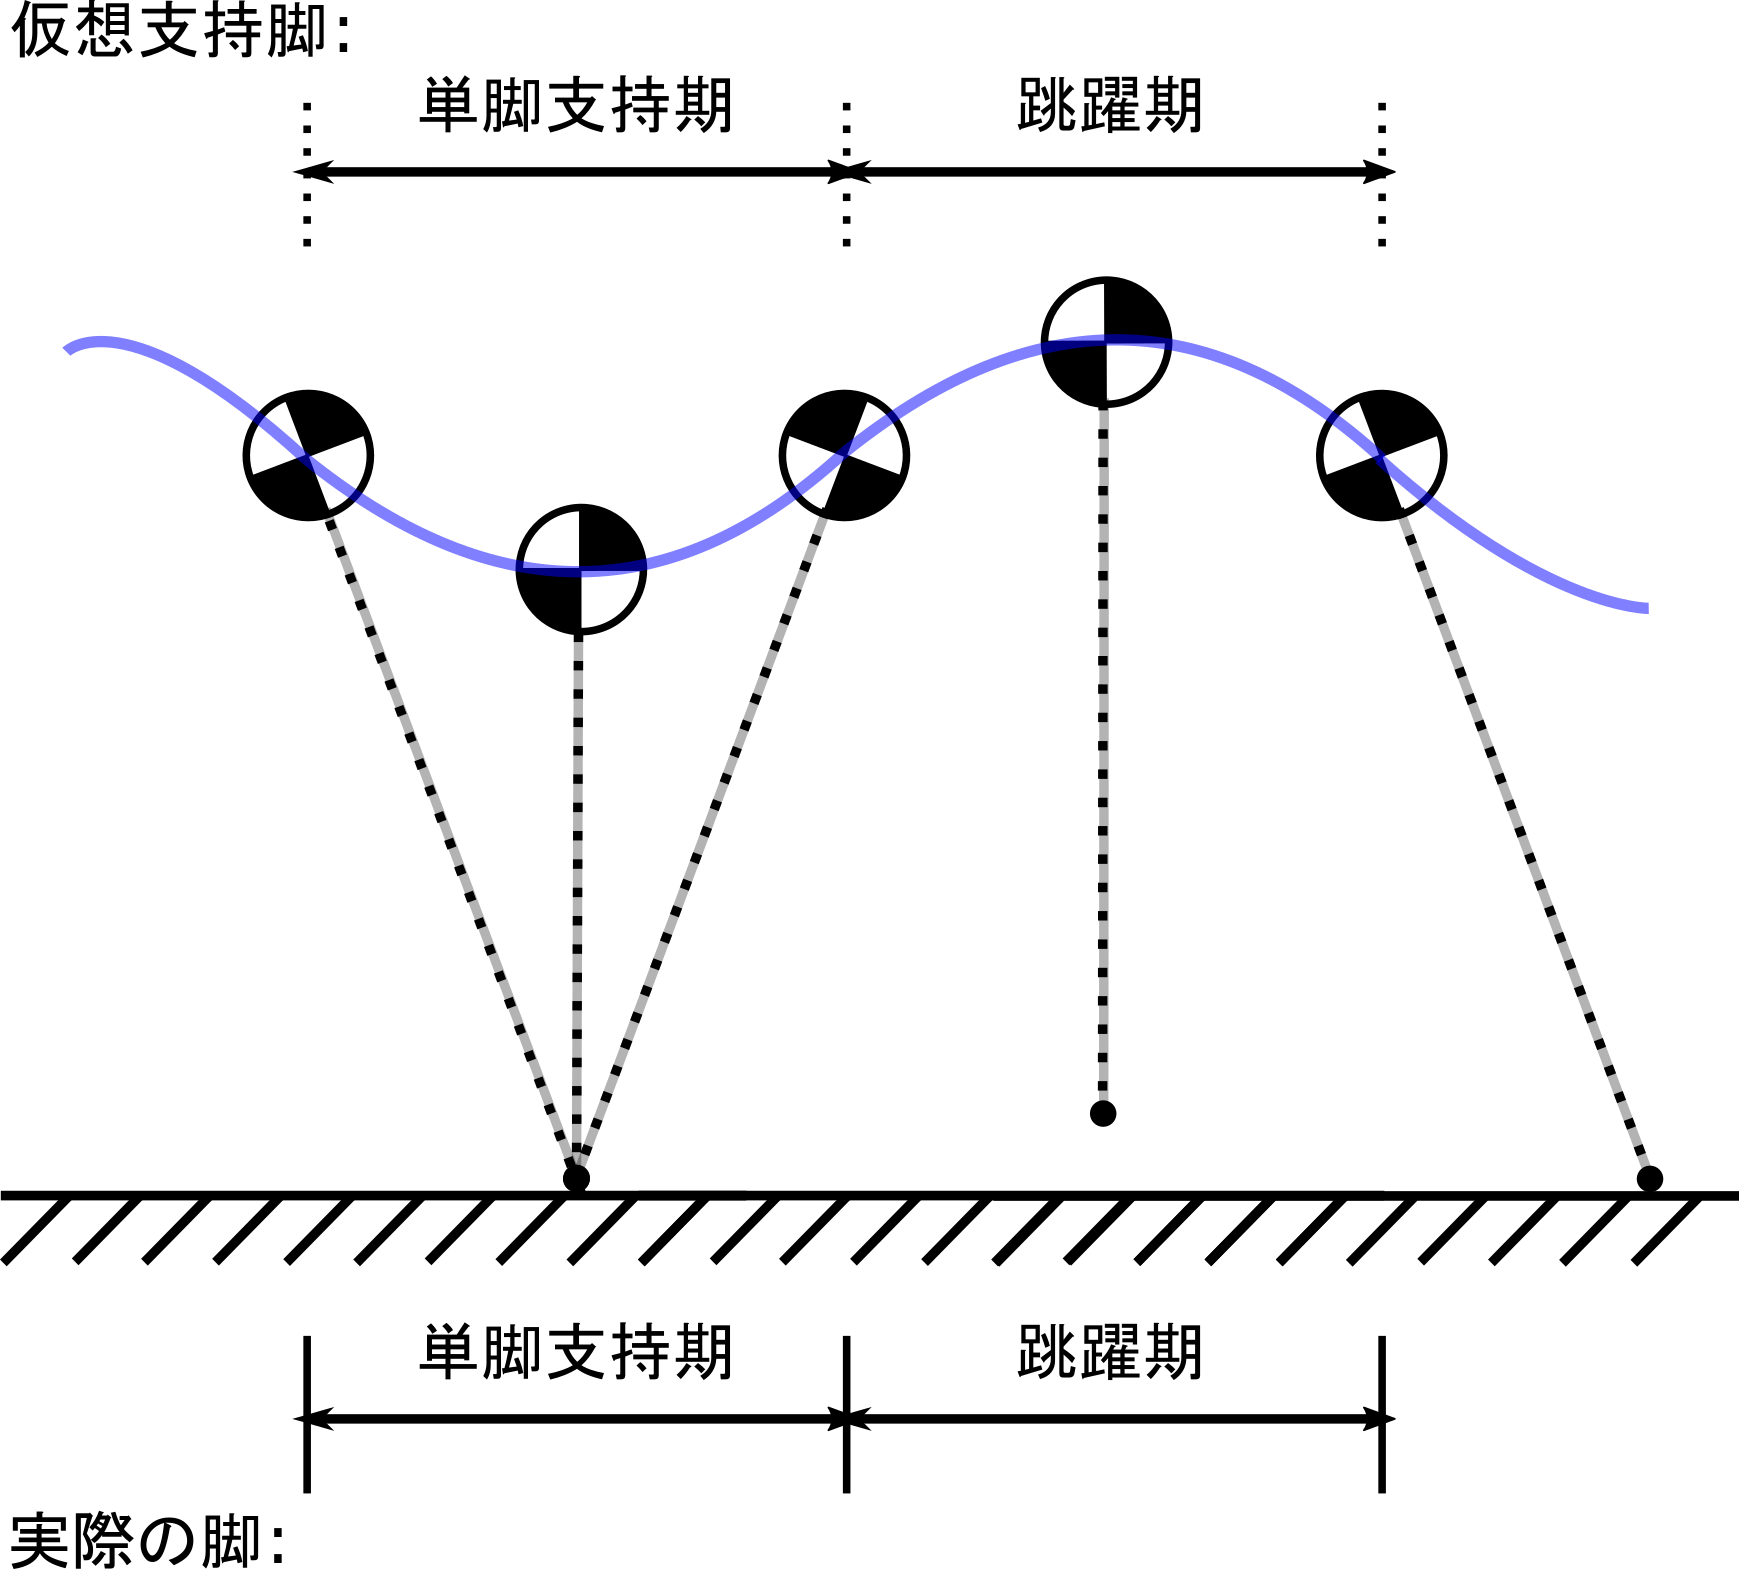
\includegraphics[width = 10.0cm,clip]{./fig/running_with_vsl.png}
 \caption{走行動作に仮想脚を導入した場合.歩行の場合と同様に,青色の曲線は重心軌跡を,黒色の線は脚を,黒色の点線は仮想脚を表している.\label{r_vsl}}
\end{figure}

\begin{figure}[htbp]
 \centering
 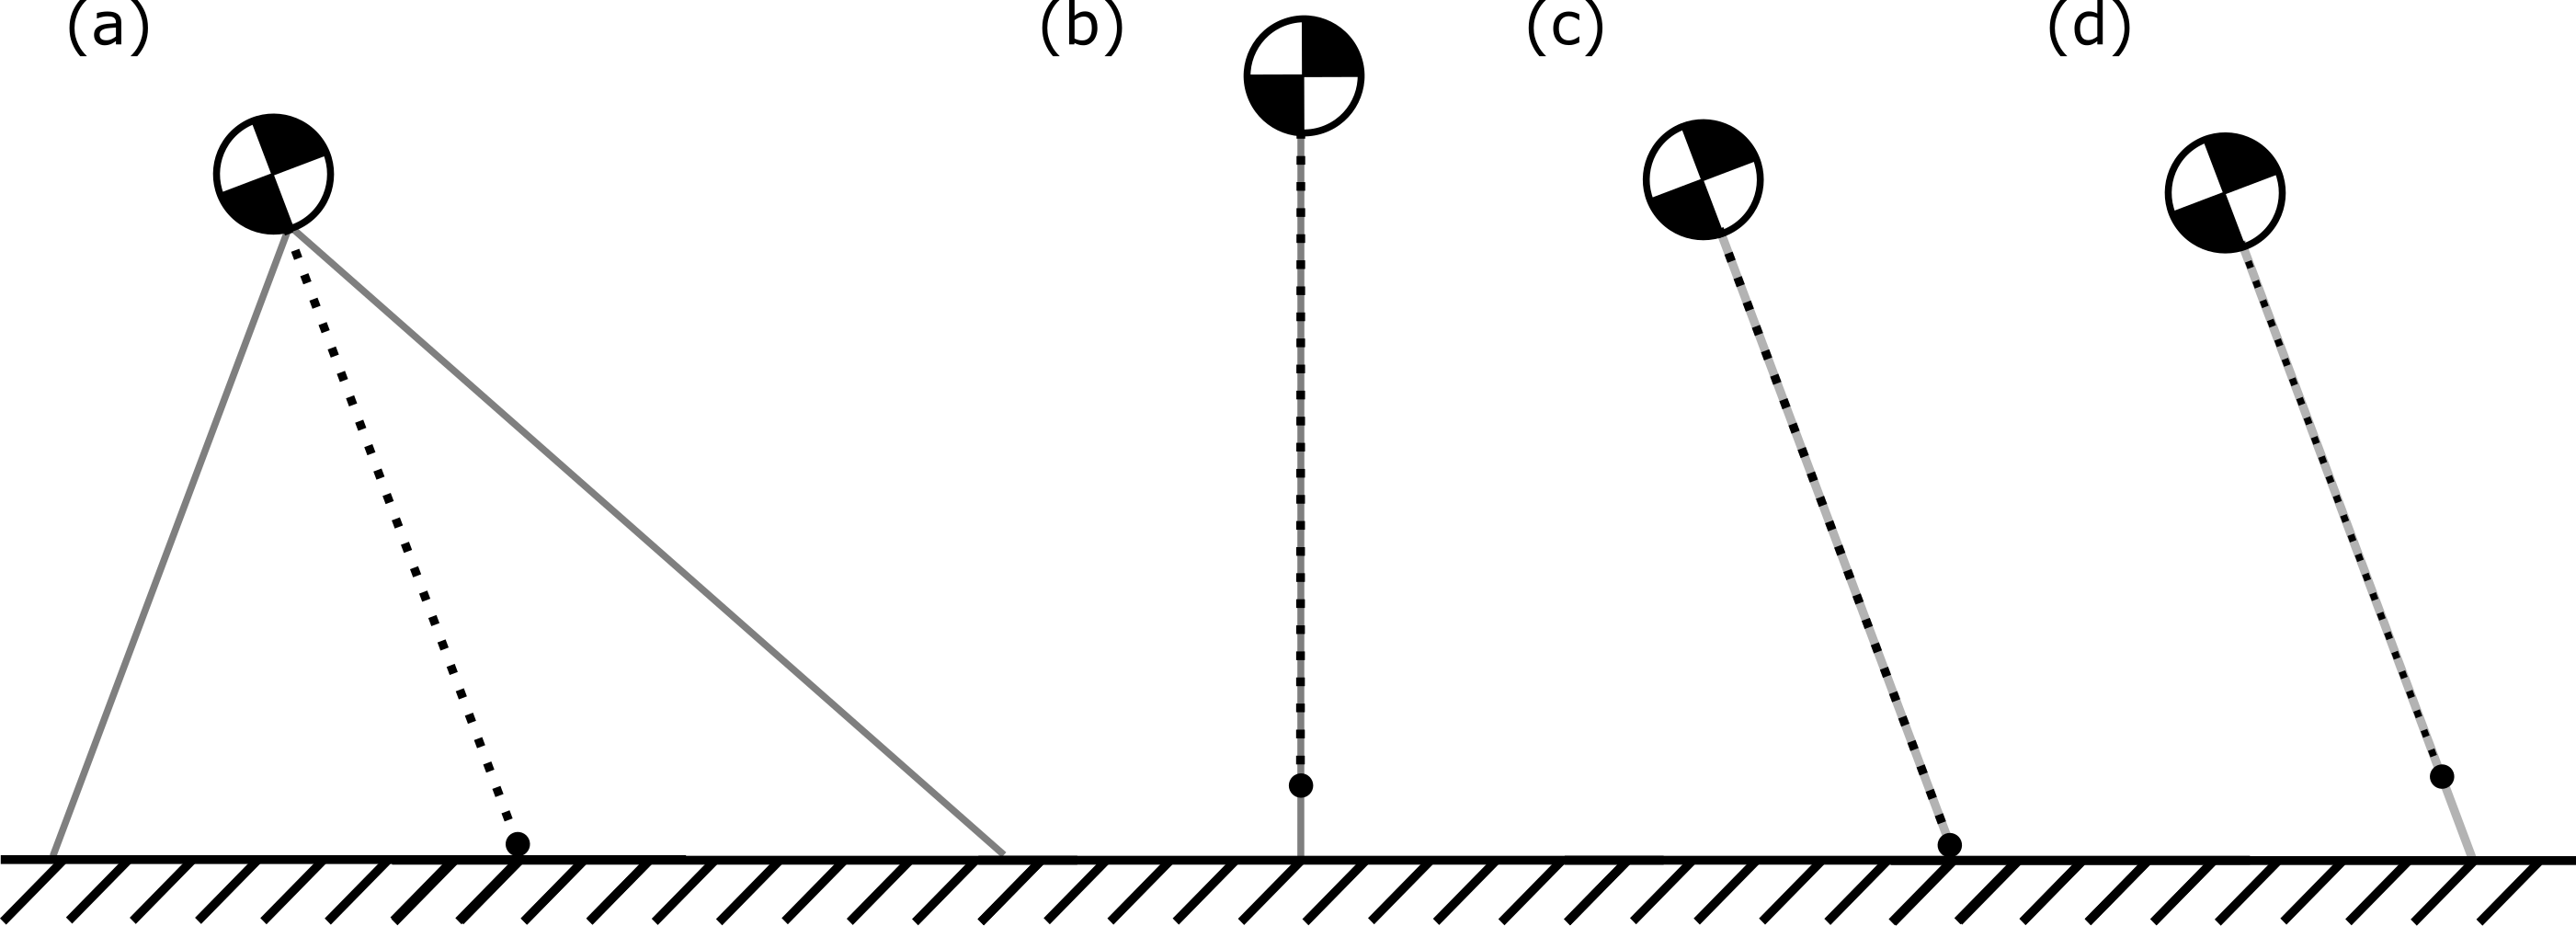
\includegraphics[clip,width=12.0cm]{./fig/vsl_pattern.png}
    \caption{仮想脚と実際の脚がとりうる状態.\label{compare}}
\end{figure}

\begin{table}[htbp]
 \centering
 \begin{tabular}{|l||c|c|c|c|} \hline
     & (a) & (b) & (c) & (d) \\ \hline \hline
    実際の脚 & 両脚支持 & 跳躍 & 単脚支持 & 単脚支持 \\
    仮想脚 & 単脚支持 & 跳躍 & 単脚支持 & 跳躍 \\
 \end{tabular}
\end{table}



\subsection{シミュレーション}

シミュレーションにおける条件として,質量体の質量80[kg],最大時の脚長1.0[m],仮想脚長0.96[m],ばね定数100000[N/m],ダンパ定数1000[Ns/m],目標高さ0.98[m]とし,ばねは脚長が0.97[m]未満のとき作用し,ダンパは現実環境では常に減衰作用が働くことを考慮して,脚長に関わらず作用するようにした.
また,初期条件として,重心位置は水平方向には0[m],鉛直方向には0.2[m]から,水平方向に目標速度を与えた状態で開始する.
この条件で,目標水平速度のみを変化させたときの歩容の変化,重心軌道,水平速度と鉛直速度の推移を観測した.
また,このときの目標水平速度は,0.5m/sから2.0m/sまで,0.5m/sづつ変更することで,モデルの運動の変化を計測した.

以下に,シミュレーションの結果を示す.
Fig.\ref{dx05}とFig.\ref{dx20}はそれぞれ,提案したモデルによる歩行と走行の運動の様子を表している.
また,Fig.\ref{trjdx05}とFig.\ref{trjdx20}はそれぞれ,歩行中,及び走行中の重心軌跡を表している.
横軸,縦軸はそれぞれ水平方向の移動量[m],高さ[m]を表している.

シミュレーションの結果,提案したモデルの目標水平速度を変更するだけで,歩容の遷移が可能であることがわかった.
本実験におけるパラメータでは,目標水平速度1.3[m/s]を境にして,歩行から走行に歩容が変化した.
走行動作においては,いずれの目標水平速度を与えた場合でも,安定な走行状態に収束し,モデルの重心軌道や鉛直方向・水平方向の速度軌跡が一定の波形に収束することがわかった(Fig.\ref{rtrj}).
歩行動作は,走行動作と比較すると,速度軌跡の収束にやや遅れや乱れが見られるものの,走行動作の場合と同様に,重心軌道や速度軌道が一定の波形に収束することができることがわかった(Fig.\ref{wtrj}).




\begin{figure}[htbp]
 \centering
 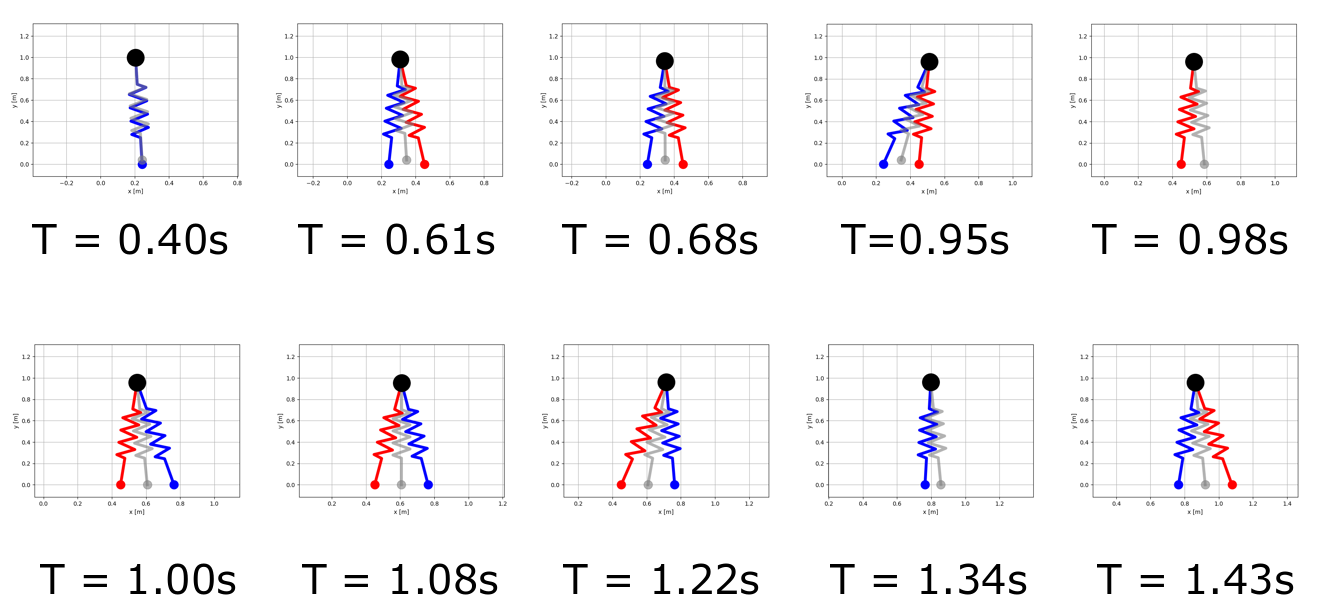
\includegraphics[width = .85\linewidth, clip]{./fig/dx0_5_walking.png}
 \caption{目標水平速度0.5m/sの場合のシミュレーション.\label{dx05}}
\end{figure}
\begin{figure}[htbp]
 \centering
 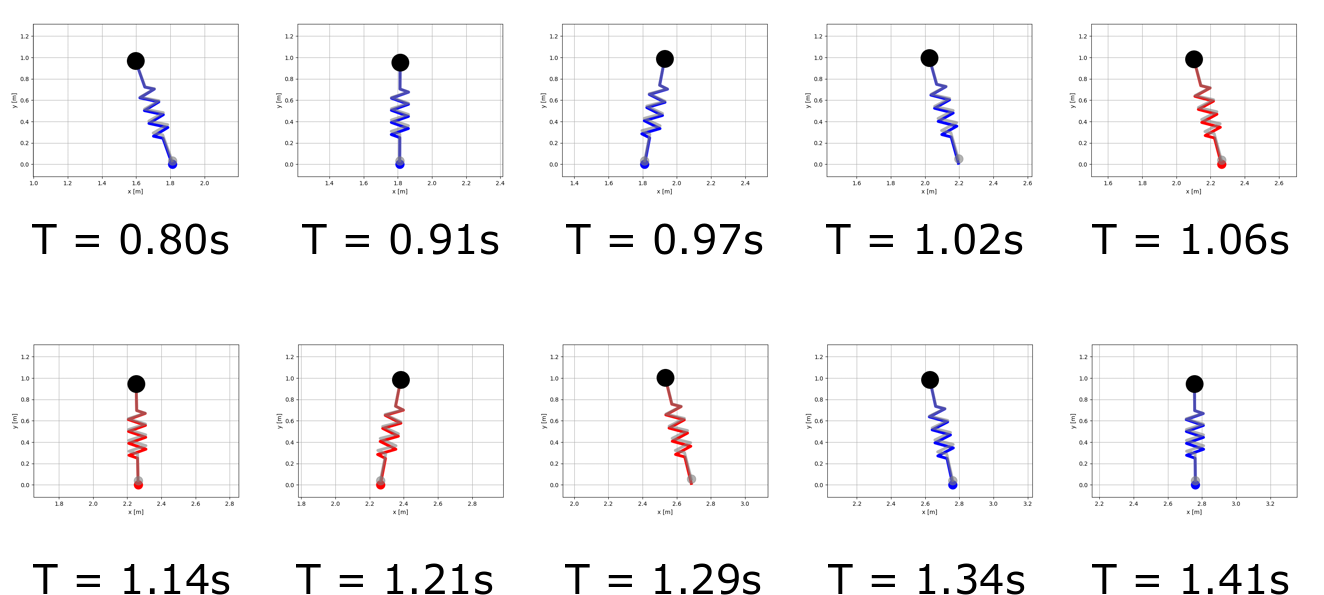
\includegraphics[width = .85\linewidth, clip]{./fig/dx2_0_running.png}
 \caption{目標水平速度2.0m/sの場合のシミュレーション.\label{dx20}}
\end{figure}
\begin{figure}[htbp]
 \begin{minipage}[b]{.5\linewidth}
 \centering
 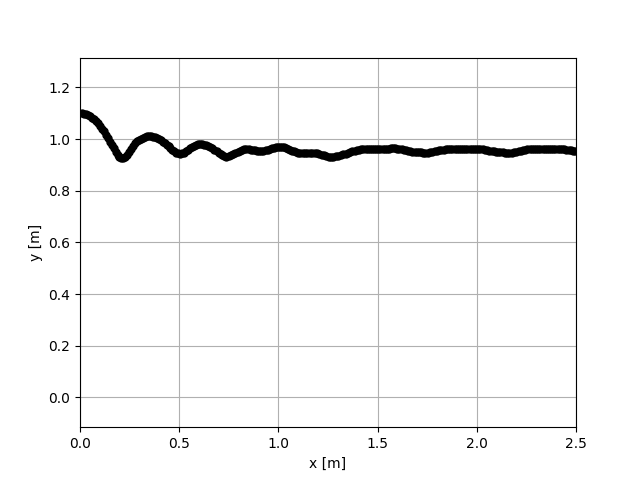
\includegraphics[width = 8cm, clip]{./fig/trj_x2_5_dx1.png}
 \caption{目標水平速度0.5m/s(歩行)の場合の重心軌跡.\label{trjdx05}}
 \end{minipage}
 \begin{minipage}[b]{.5\linewidth}
 \centering
 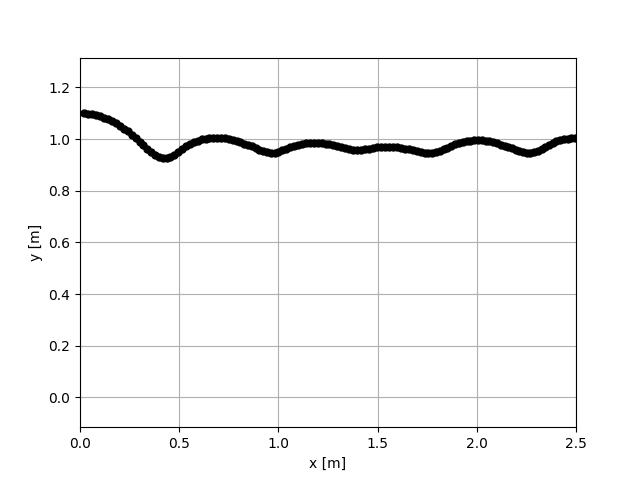
\includegraphics[width = 8cm,clip]{./fig/trj_x2_5_dx2.png}
 \caption{目標水平速度2.0m/s(走行)の場合の重心軌跡.\label{trjdx20}}    \end{minipage}
\caption{歩行と走行における重心軌跡.\label{trj}}
\end{figure}


\begin{figure} % 仮
 \begin{minipage}[b]{.5\linewidth}
  \centering
  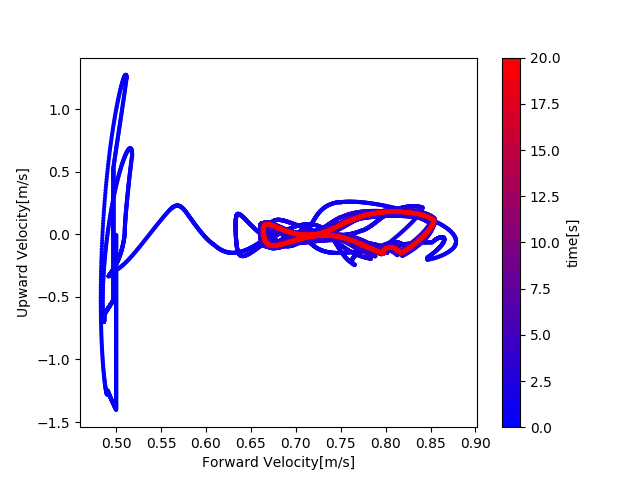
\includegraphics[clip,width = 8cm]{./fig/Velocity_dx0_5walk.png}
  \subcaption{目標水平速度0.5m/sの場合の速度軌跡\label{dxtrj_dx05}.}
 \end{minipage}
 \begin{minipage}[b]{.5\linewidth}
  \centering
  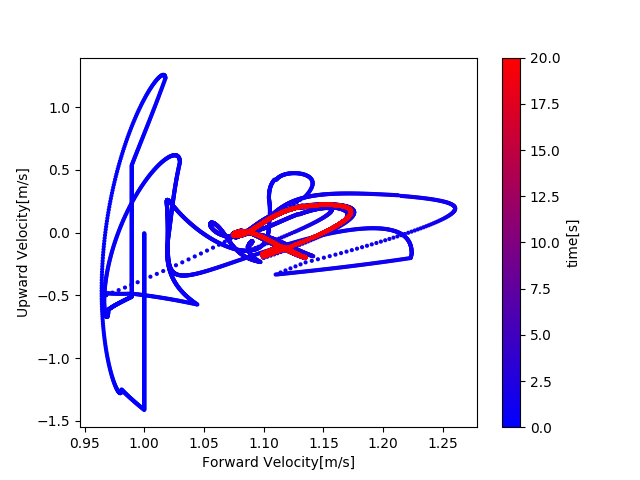
\includegraphics[clip,width = 8cm]{./fig/Velocity_dx1walk.png}
  \subcaption{目標水平速度1.0m/sの場合の速度軌跡\label{dxtrj_dx10}.}
 \end{minipage}
 \caption{歩行時の速度軌跡.\label{wtrj}}
 \begin{minipage}[b]{.5\linewidth}
  \centering
  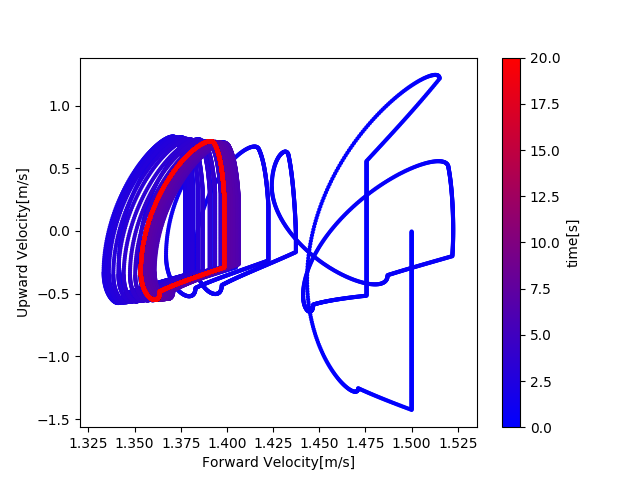
\includegraphics[clip,width = 8cm]{./fig/Velocity_dx1_5run.png}
  \subcaption{目標水平速度1.5m/sの場合の速度軌跡\label{dxtrj_dx15}.}
 \end{minipage}
 \begin{minipage}[b]{.5\linewidth}
  \centering
  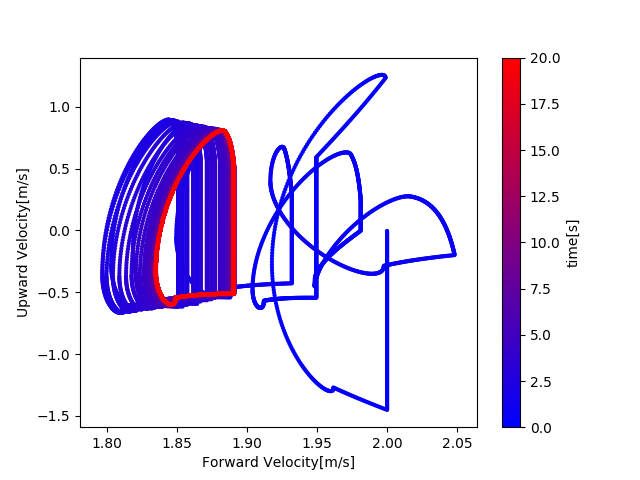
\includegraphics[clip,width = 8cm]{./fig/Velocity_dx2run.png}
  \subcaption{目標水平速度2.0m/sの場合の速度軌跡\label{dxtrj_dx20}.}
 \end{minipage}
 \caption{走行時の速度軌跡.\label{rtrj}}
\end{figure}
